\subsection{Comparison to the original system} \label{section:comparisontooriginal}

As mentioned before, the service aims to provide roughly the same functionality as the original system by Blocket with some improvements and extensions. The semantics of transfer of goods work in roughly the same manner, as was described in the discussion about the original service in Figure \ref{fig:agreementaction} (can be compared to the state machine from Figure \ref{fig:dfa}). However, there are some differences, which address some of the concerns, related to the original system. It is also important to note, that some of the improvements and extensions introduced some other potential drawbacks.

\subsubsection{All-in-one interface}
In comparison to the original system, the application, which was developed in this thesis work provides an all-in-one (AIO) interface. Modules, such as conflict resolving, trading of merchandise, explorer of addresses and logistics process monitoring are all integrated into one easy-to-use interface, which could not be said about the original system.

\subsubsection{Sensor support} \label{section:sensorsupported}
Sensor support is not provided in the original system. The discussion about how the integration of sensor functionality would potentially benefit a merchandise trading platform was provided in Sections \ref{section:additional functionality} and \ref{section:features}, as well as in user stories, which were described in Section \ref{section:userstories}. However, the introduction of sensor support is both problematic to implement in the real world and can also introduce some trust-related issues.

\paragraph{Infrastructure absence}
There currently is no infrastructure that supports real-time sensor communication, during the logistics process. Parcel tracking is a very common functionality among logistics companies nowadays, however, this functionality is very trivial and parcels' positions are only updated once the they pass through logistics company's sorting facilities. 

Even though this thesis work focuses mainly on the software side, it is important to keep in mind that the infrastructural challenges, which have to dealt with in order to make real-time sensor communication possible, are huge. Each individual sensor needs to be able to communicate with the application and regularly send updated sensor readouts on the move through the landscape, which is very challenging to achieve.

Assuming that the parcels are transported, using road-going vehicles, such as delivery trucks, the possible solution to that problem is to use the cellular network infrastructure for sensor data communication. Cellular networks is a fast evolving sphere of information technologies with 5G already being tested by tech giants, such as Nokia, Ericsson and Huawei \citep{5gtesting}. The necessary factor for making this approach work is the degree and extent of cellular network coverage. In Sweden, most of inhabited municipalities and highways between cities possess very good 3G and 4G coverage, as shown in Figure \ref{fig:4gcoverage}. 

\begin{figure}[H]
\centering
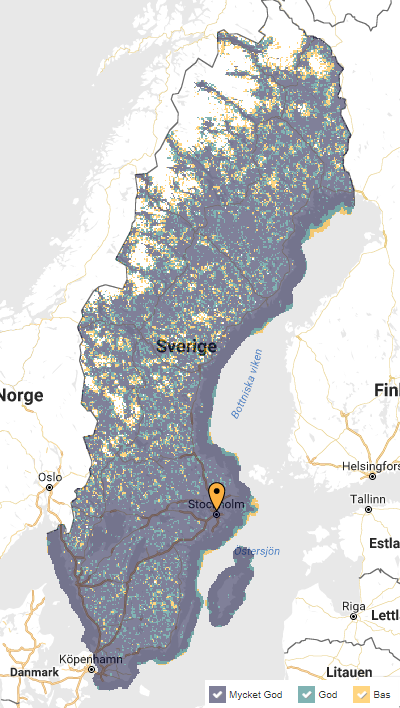
\includegraphics[scale=0.68]{images/4gcoverage.png}
\caption{Cellular mobile network coverage of Sweden's largest mobile service provider, Telia (2G, 3G, 4G and 4G+). Blueish areas on the map have excellent coverage, greenish areas have good coverage and yellowish areas possess basic coverage \textnormal{\citep{teliacoverage}}.}
\label{fig:4gcoverage}
\end{figure}

Theoretically, the approach of using cellular networks is rather possible (at least as far as Sweden is considered), due to extremely good cellular coverage of the country. However, in order to make this approach happen, each  road-going delivery vehicle and parcel sorting facility would need to be fitted with a central sensor data processing unit, as well as a 4G transmitter. All of this hardware would turn out being rather pricey for the logistics companies, as thousands of such processing units and transmitters would need to be installed. It all depends on the logistics companies being willing to commit such large amounts of resources on that functionality, and if they would, I assume that the inclusion of sensors would turn out being a rather costly service for the users, as companies would then try to earn the spent money back, by charging a hefty price for sensor inclusion. Visualization of that approach is displayed in Figure \ref{fig:sensorinfrastructure}.

\begin{figure}[H]
\centering
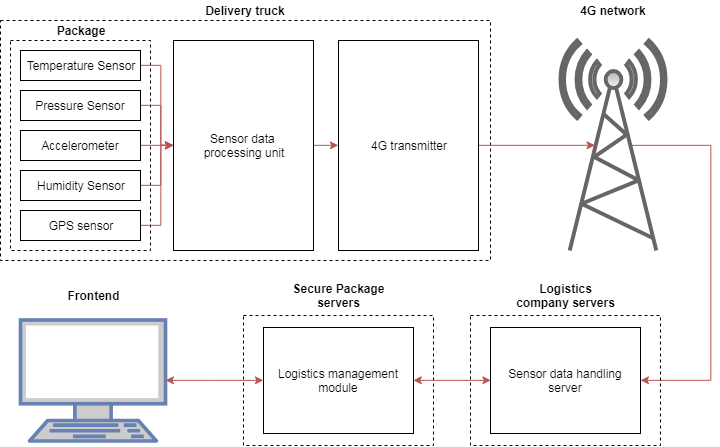
\includegraphics[scale=0.5]{images/infrastructuresensor.png}
\caption{Potential infrastructure model for integration of server support.}
\label{fig:sensorinfrastructure}
\end{figure}

\paragraph{Sensor-related trust issues}
It is important to keep in mind that logistics company is the party who is to provide and maintain the sensors and its infrastructure. Even though the sensors might be working as they should, a logistics company might theoretically implement a server backend module, that performs manipulations on incoming sensor output values to make them not exceed the configured thresholds of the parcels, in case of detected violations. Thus this module would allow the logistics companies to violate the terms of transfer without generating any violation events. 

Another possible fraud, that could be performed by the logistics company is that the sensor data processing unit from the potential infrastructure model, which was shown in Figure \ref{fig:sensorinfrastructure}, would be extended with a functionality of simulating sensor values before sending them to the sensor data handling server. This would theoretically make it possible to remotely turn off all the sensors during the transport process and simulate sensor data with faulty values that would not generate any (or, to make it more trustworthy, a few) violations.

In order to prevent those frauds from happening, regular audits would need to be performed by a trusted authority.

\paragraph{Faulty sensors}
The following scenario is also relevant for the discussion about clerk resolving. Consider, that an expensive antique mirror was sold, using the centralized Secure Package. Buyer and seller came to an agreement that an accelerometer should be sent along with the mirror, as it is very fragile when it comes to sudden drops. The parcel with the mirror was then shipped, but the sensor stopped working during the transfer process. Then, the mirror breaks due to being dropped by an employee during the unloading process. Now, the question is: \textit{"can the parties prove that it was all logistics company's fault, without a working sensor?"}. There is little to no way of proving that the mirror was not destroyed before being shipped, which makes the conflict resolving process of that case extremely tricky.

Another fact to consider is that, sometimes, sensors tend to show faulty values. A simple calibration could potentially fix that, however, what should the regulations be, in case of the parcel's contents being damaged and sensors showing incorrect values that should have, but didn't generate a violation event? Those extreme cases would need to be considered in case of implementing this technology in the real world.

\subsubsection{Bidding auction principal}
The principal of agreement establishment is different, compared to the the original system, in a way that the centralized Secure Package provides an auction-like principal. Potential buyers are proposing their terms, allowing the seller to pick the best one (probably the one with highest amount of money). This favors the sellers, as they can potentially get more money for their items.

It is important to consider that money is not the only decisive factor of the bidding process. The other factors, such as sensor selections and logistics deadline, can potentially be more important to users in some cases.

\subsubsection{Conflict resolving}
Clerk resolving is a very controversial subject in context of this project. In the early phases of this work, I tried reaching Blocket in order to get more information about the conflict resolving principal, which is used in their application. Unfortunately, I did not get a reply on my e-mail message. I have no previous experience with having to deal with a purchase conflict myself, thus I don't have any information on what procedures are used by Blocket. 

\paragraph{Buyer's advantage in case of a conflict}
There are some potential cases, which would be tricky to resolve, disregarding the conflict resolving policies. For example, consider following case:

\begin{itemize}
\item Seller sells a laptop to some buyer, using a merchandise trading platform.
\item Sellers sends the package with a laptop to the buyer.
\item Laptop arrives in good condition.
\item Buyer decides to scam the seller by disapproving the condition of the item, keeping the fully functional laptop and sending back a brick (or something else of no value).
\item Seller receives the return and is very surprised when he discovers that the returning parcel contained a brick. Seller generates a conflict request.
\end{itemize}

It would be very difficult to prove the fact that the seller did not initially send a brick. This makes the whole mechanism of using such merchandise trading platforms quite risky for the sellers. In other words, theoretically, buyers have much more confidence in such a system, then sellers do.

\paragraph{Trustworthiness of clerks}
In the original system, it is obvious that Blocket themselves handle conflict resolving. This introduces a problem, as the clerk administrator could potentially be biased towards Blocket (as the administrator himself is Blocket employee), as well as the logistics company DBSchenker, as Blocket and DBSchenker are partners. Therefore, this was the reason why the trusted legal authority, that has no relations to the organization, that runs the service, and to the logistics company, was proposed for conflict resolving purposes of the centralized Secure Package.

\subsubsection{Increased overall trust}

In comparison to the original system, the centralized Secure Package system may be considered being more trustworthy, due to its increased transparency, which is provided by introduction of the explorer module, and privacy aspects, which is achieved by protection of private information. Increased transparency significantly lowers the chance of undetected scams, performed by the organization, that runs the service, as all of the agreement-related events are made public, which introduces tracing functionality. Privacy and anonymity are very important aspects to some users, that are very careful about who they share their private information with. Increased privacy lowers probability of potential identity frauds.

